\FloatBarrier
\begin{figure}[!h]
\centering
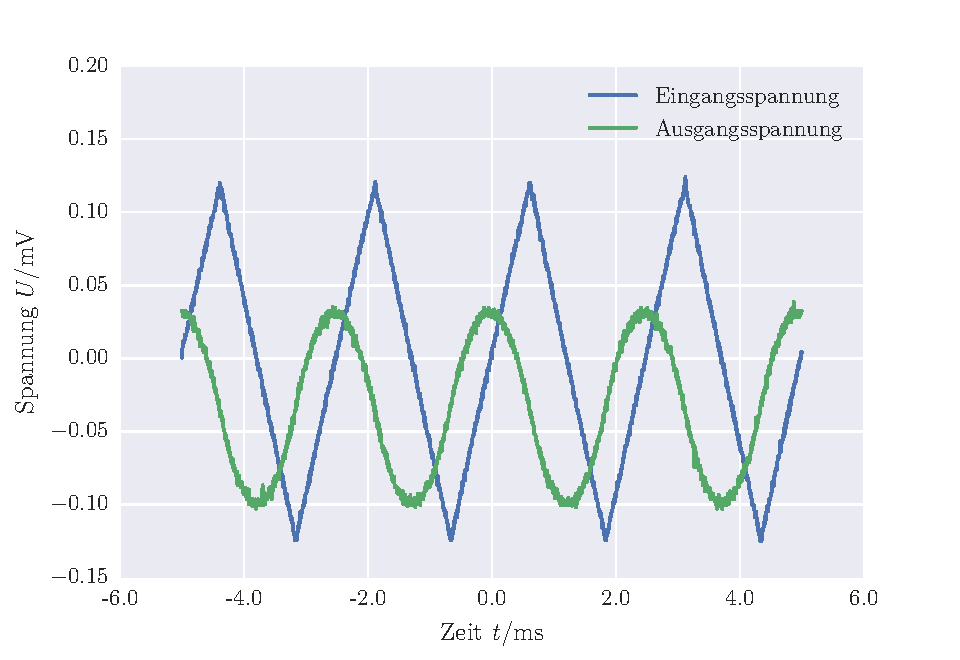
\includegraphics[scale=0.75]{../Grafiken/Integrator_Oszilloskop_Dreieck.pdf}
\caption{Vom Oszilloskop aufgenommene Ein- und Ausgangsspannungen der Integratorschaltung. Auf dem Eingang
	liegt hier eine Dreicksspannung. Die Ausgangsspannung in Form entspricht dem theoretisch
	zu erwartendem Verlauf (periodische Abfolge nach oben respektive nach unten geöffneter 
	Parabeln).\label{fig:integrator_oszilloskop_dreieck}}
\end{figure}
\FloatBarrier